\documentclass{article}

\usepackage{graphicx}
\usepackage{xcolor}
\usepackage{subcaption}
\usepackage{indentfirst}
\usepackage[a4paper, total={6in, 8in}]{geometry}
\usepackage{hyperref}
\usepackage{fancyhdr}
\usepackage{xepersian}
\settextfont{B Nazanin}
\setlatintextfont{Times New Roman}

\definecolor{codegray}{gray}{0.9}
\newcommand{\code}[1]{\colorbox{codegray}{\texttt{\lr{#1}}}}

\begin{document}


%title page%
\begin{titlepage}
	\begin{center}
		\vspace{0.2cm}
		
		
\includegraphics[width=0.4\textwidth]{sharif.png}\\
		\vspace{0.2cm}
		\textbf{ \Huge{آزمایش شماره 7}}\\
		\vspace{0.25cm}
		\textbf{ \Large{آز شبکه - دکتر بردیا صفایی}}
		\vspace{0.2cm}
		
		
		\large \textbf{دانشکده مهندسی کامپیوتر}\\\vspace{0.1cm}
		\large   دانشگاه صنعتی شریف\\\vspace{0.2cm}
		\large   ﻧﯿﻢ‌سال اول ۰۱-۰۲ \\\vspace{0.10cm}
		\large{ گروه 8:}\\
		\large{\href{mailto:mehrshad.mirmohammadi@gmail.com}{مهرشاد میرمحمدی - 98109634}}\\
		\large{\href{mailto:parhaamsaremi@gmail.com}{پرهام صارمی - 97101959}}\\
		\large{\href{mailto:mofayezi.m@gmail.com}{محمدرضا مفیضی - 98106059}}\\
	\end{center}
\end{titlepage}
%title page%

\newpage

%pages header
\pagestyle{fancy}
\fancyhf{}
\fancyfoot{}
\setlength{\headheight}{59pt}
\cfoot{\thepage}
\lhead{آزمایش شماره 7}
\rhead{
\includegraphics[width=0.1\textwidth]{sharif.png}\\
		دانشکده مهندسی کامپیوتر
}
\chead{آز شبکه - گروه 8}
%pages header

 در این آزمایش به پیاده‌سازی سه سناریو مطرح شده در کلاس می‌پردازیم.
 \section{سناریو اول}
 سناریو اول را مطابق شکل \ref{fig:s-1} پیاده می‌کنیم.
 \begin{figure}[h!]
 	\centering
 	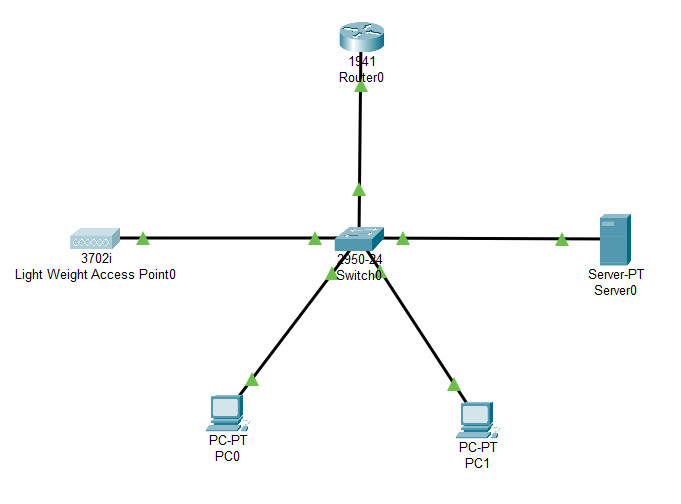
\includegraphics[width=0.5\columnwidth]{figs/s-1.jpg}
 	\caption{سناریو اول در محیط \lr{packet tracer}}
 	\label{fig:s-1}
 \end{figure}

ابتدا به سرور \lr{DHCP} آدرس می‌دهیم ولی به \lr{PC} ها آدرس نمی‌دهیم چون باید توسط \lr{DHCP} آدرس‌دهی شوند. سپس به روتر آدرس می‌دهیم(شکل \ref{fig:s-1-router-add}) و همچنین با دستور \code{ip helper-address} آدرس ایستای سرور را برای آن تعریف می‌کنیم. (شکل \ref{fig:s-1-router-helper-add})

\begin{figure}[h!]
	\centering
	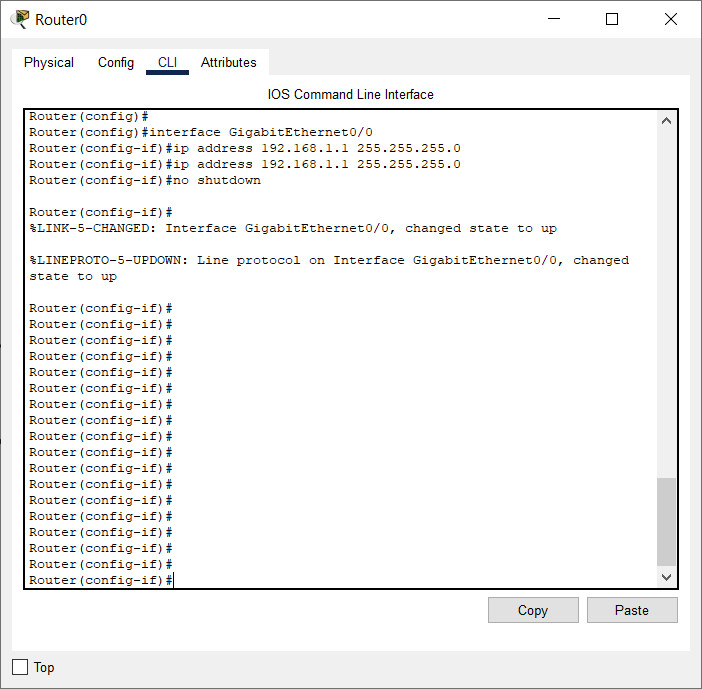
\includegraphics[width=0.5\columnwidth]{figs/s-1-router-add.jpg}
	\caption{آدرس‌دهی روتر}
	\label{fig:s-1-router-add}
\end{figure}

\begin{figure}[h!]
	\centering
	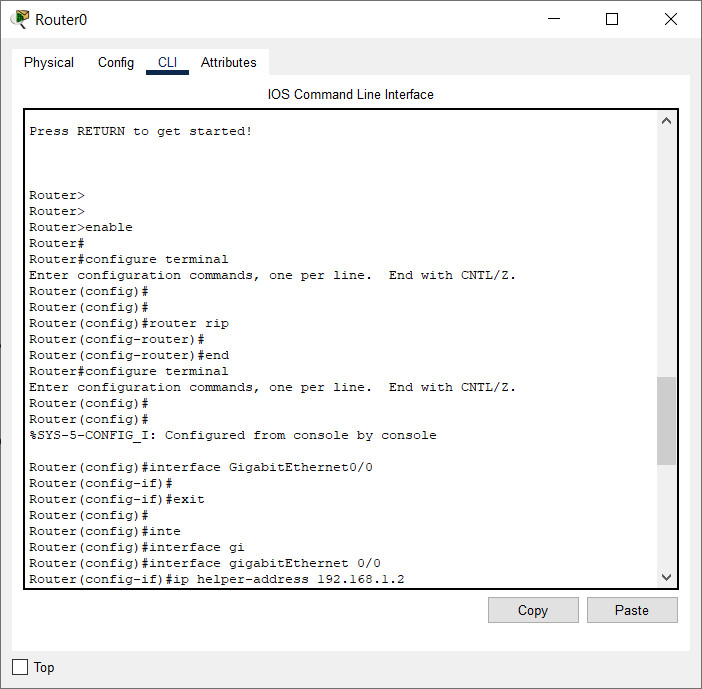
\includegraphics[width=0.5\columnwidth]{figs/s-1-router-helper-add.jpg}
	\caption{تعیین آدرس ایستای سرور \lr{DHCP}}
	\label{fig:s-1-router-helper-add}
\end{figure}

با رفتن به بخش \lr{Services} سپس \lr{DHCP} در سرور، تنظیمات را انجام می‌دهیم.
حالا \lr{ip pool} را مطابق شکل \ref{fig:s-1-server-pool} اضافه می‌کنیم.
 \begin{figure}[h!]
	\centering
	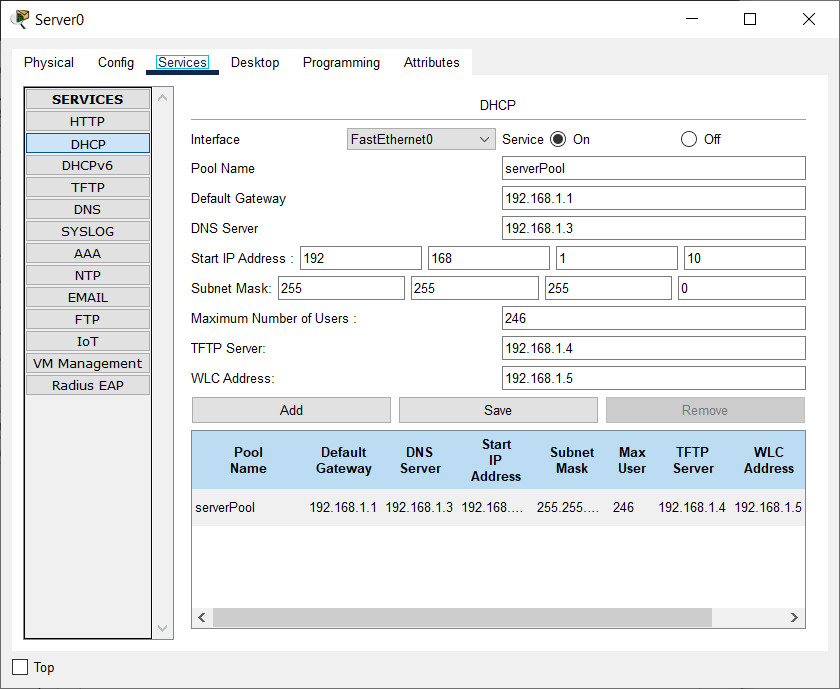
\includegraphics[width=0.5\columnwidth]{figs/s-1-server-pool.jpg}
	\caption{\lr{ip pool} اضافه شده در سرور}
	\label{fig:s-1-server-pool}
\end{figure}

درنهایت با تغییر \lr{ip configuration} در \lr{PC} ها آدرس آن‌ها توسط \lr{DHCP} مطابق شکل‌های \ref{fig:s-1-pc} مقداردهی خواهد شد. همچنین در \lr{light weight access point} مقدار \lr{primary controller} (شکل \ref{fig:s-1-ap}) و آدرس تعیین خواهد شد.
\begin{figure}
	\centering
	 \begin{subfigure}{.4\columnwidth}
		   \centering
		   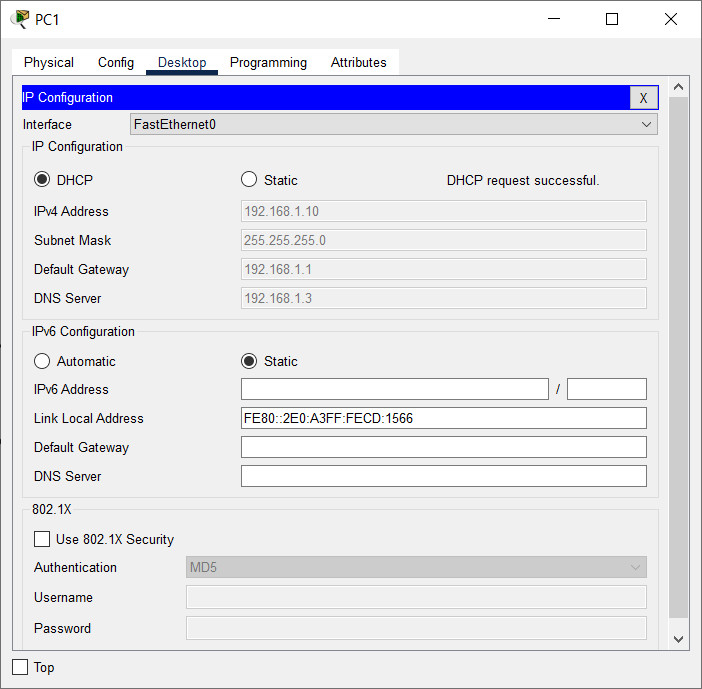
\includegraphics[width=\columnwidth]{figs/s-1-pc-1.jpg}
	\end{subfigure}%
	\begin{subfigure}{.4\columnwidth}
		\centering
		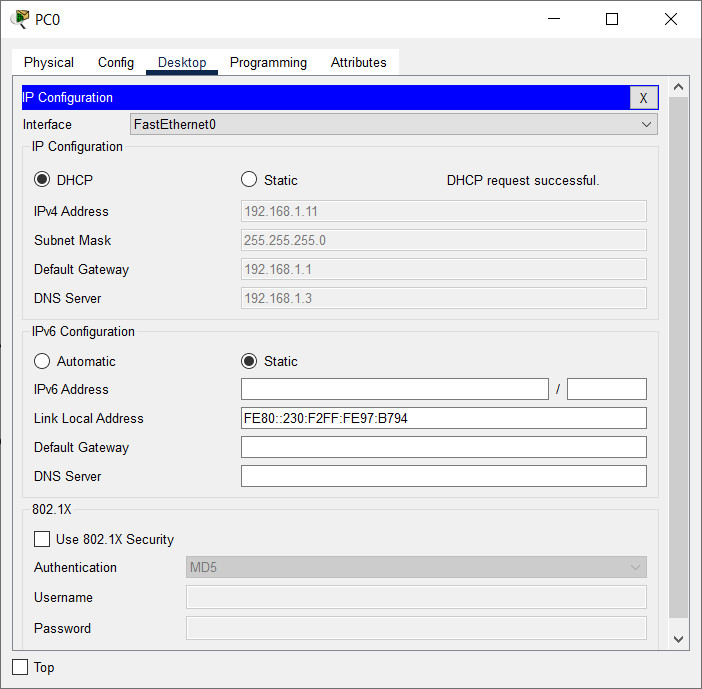
\includegraphics[width=\columnwidth]{figs/s-1-pc-2.jpg}
	\end{subfigure}
	\caption{مقادیر \lr{ip} در \lr{PC} ها}
	\label{fig:s-1-pc}
\end{figure}

 \begin{figure}[h!]
	\centering
	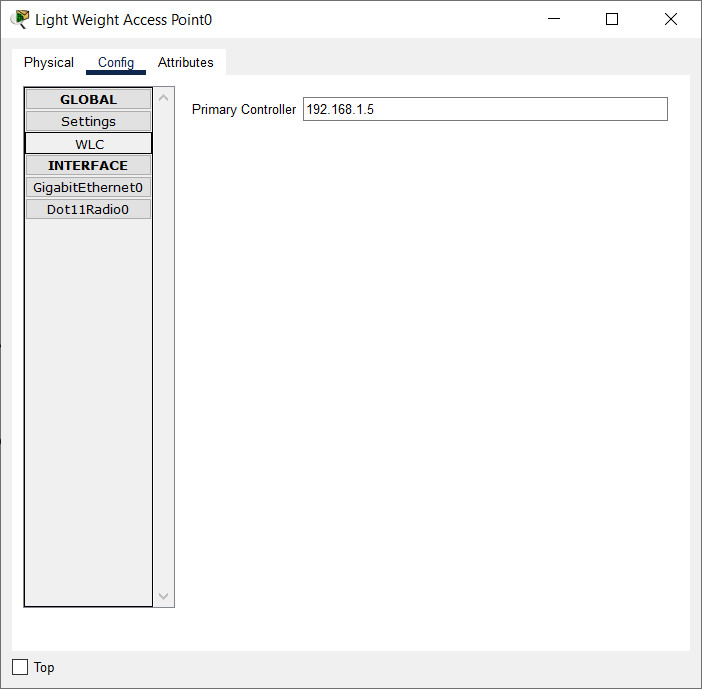
\includegraphics[width=0.5\columnwidth]{figs/s-1-ap.jpg}
	\caption{مقدار \lr{primary controller} در \lr{access point}}
	\label{fig:s-1-ap}
\end{figure}

\section{سناریو دوم}
سناریو دوم را مطابق شکل \ref{fig:s-2} پیاده می‌کنیم.
\begin{figure}[h!]
	\centering
	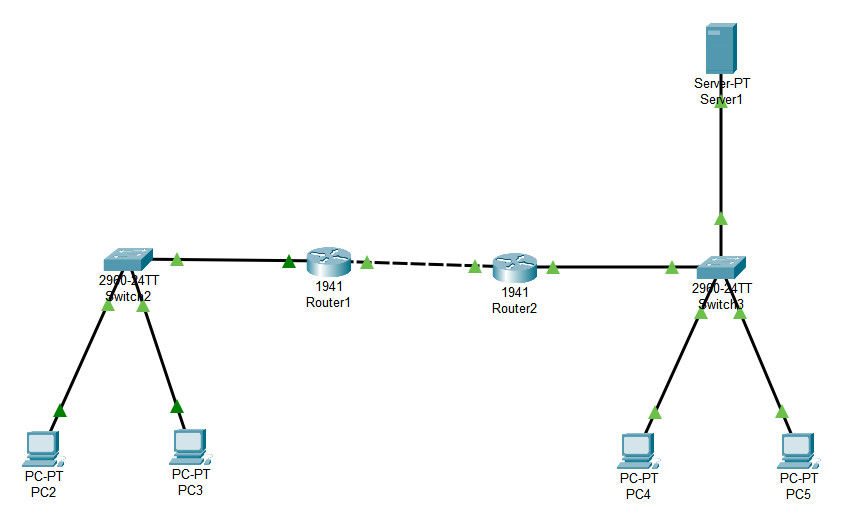
\includegraphics[width=0.5\columnwidth]{figs/s-2.jpg}
	\caption{سناریو دوم در محیط \lr{packet tracer}}
	\label{fig:s-2}
\end{figure}

ابتدا به سرور آدرس \lr{IP} و \lr{Gateway} می‌دهیم. از آنجایی که در این سناریو دو زیرشبکه داریم باید دو \lr{ip pool} در سرور ایجاد کنیم. مطابق شکل \ref{fig:s-2-server-pool} مخزن‌ها را با مشخصات داده‌شده ایجاد می‌کنیم.
 \begin{figure}[h!]
	\centering
	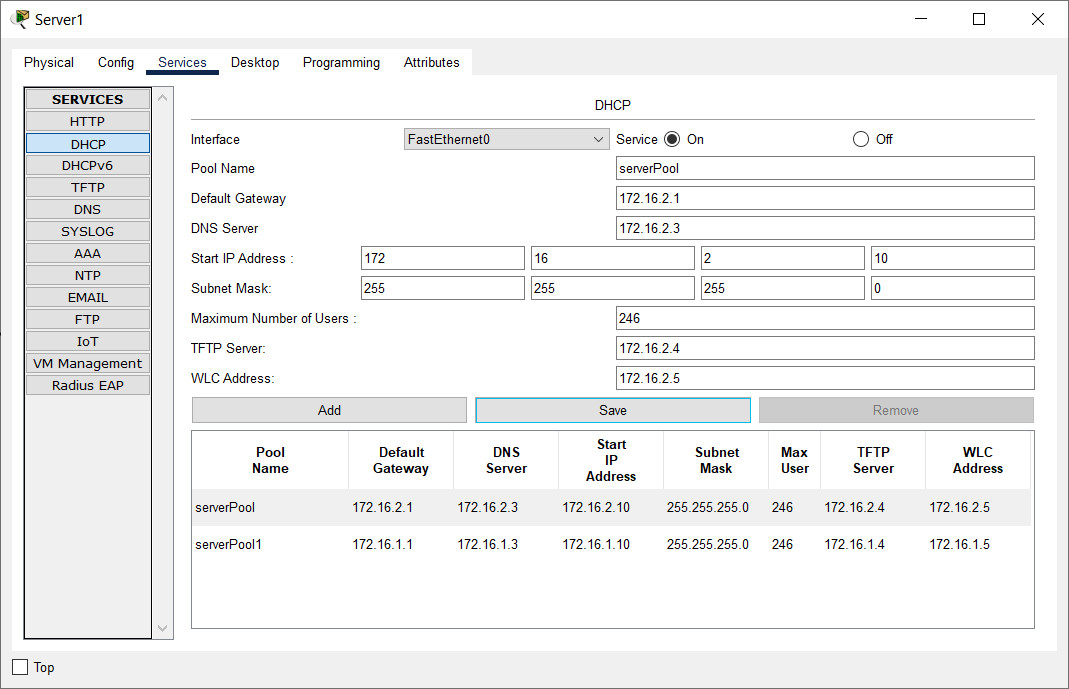
\includegraphics[width=0.5\columnwidth]{figs/s-2-server-pool.jpg}
	\caption{\lr{ip pool}های اضافه شده در سرور}
	\label{fig:s-2-server-pool}
\end{figure}

برای اتصال دو روتر از روتینگ ایستا استفاده می‌کنیم و مطابق آزمایش 4 تنظیمات را انجام می‌دهیم. حالا برای این‌که زیرشبکه سمت چپ هم بتواند به سرور \lr{DHCP} دسترسی داشته باشد باید با کمک دستور \code{ip helper-adderss} آدرس سرور \lr{DHCP} را تعیین کنیم.

درنهایت می‌بینیم که می‌توان از تمام \lr{PC} ها آدرس \lr{DHCP} را دریافت کرد. (شکل \ref{fig:s-2-pc})
\begin{figure}
	\centering
	\begin{subfigure}{.4\columnwidth}
		\centering
		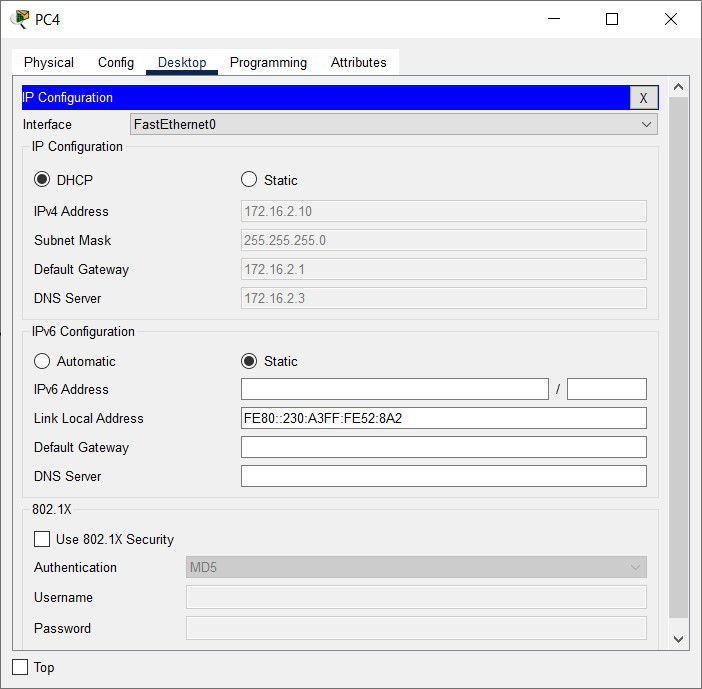
\includegraphics[width=\columnwidth]{figs/s-2-pc-1.jpg}
	\end{subfigure}%
	\begin{subfigure}{.4\columnwidth}
		\centering
		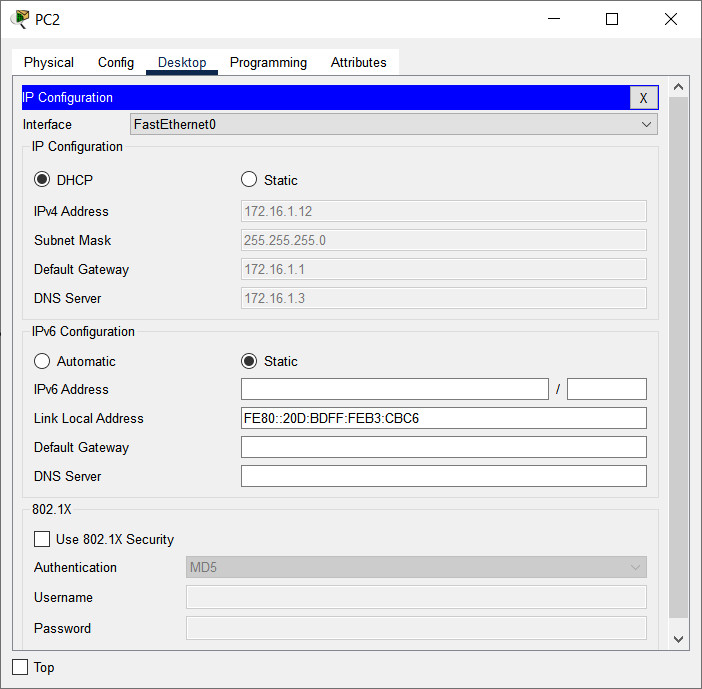
\includegraphics[width=\columnwidth]{figs/s-2-pc-2.jpg}
	\end{subfigure}
	\caption{مقادیر \lr{ip} در یکی از \lr{PC} های زیرشبکه چپ و راست}
	\label{fig:s-2-pc}
\end{figure}

\section{سناریو سوم}
سناریو سوم را مطابق شکل \ref{fig:s-3} پیاده می‌کنیم.
\begin{figure}[h!]
	\centering
	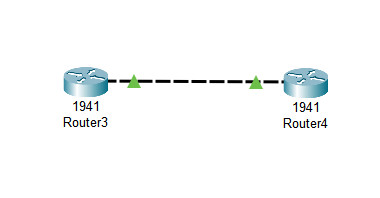
\includegraphics[width=0.5\columnwidth]{figs/s-3.jpg}
	\caption{سناریو سوم در محیط \lr{packet tracer}}
	\label{fig:s-3}
\end{figure}

از روتر سمت راست به عنوان سرور \lr{DHCP} استفاده می‌کنیم. ابتدا آدرس این روتر را به صورت ایستا تعیین می‌کنیم (دستور \code{no shutdown} هم حتما باید اجرا شود). سپس باید دستوراتی را مطابق شکل \ref{fig:s-3-router-server} برای ایجاد یک مخزن، تعیین دامنه آدرس‌های آن و تعیین \lr{default gateway} وارد کرد و روتر را به یک سرور \lr{DHCP} تبدیل می‌کنیم.
\begin{figure}[h!]
	\centering
	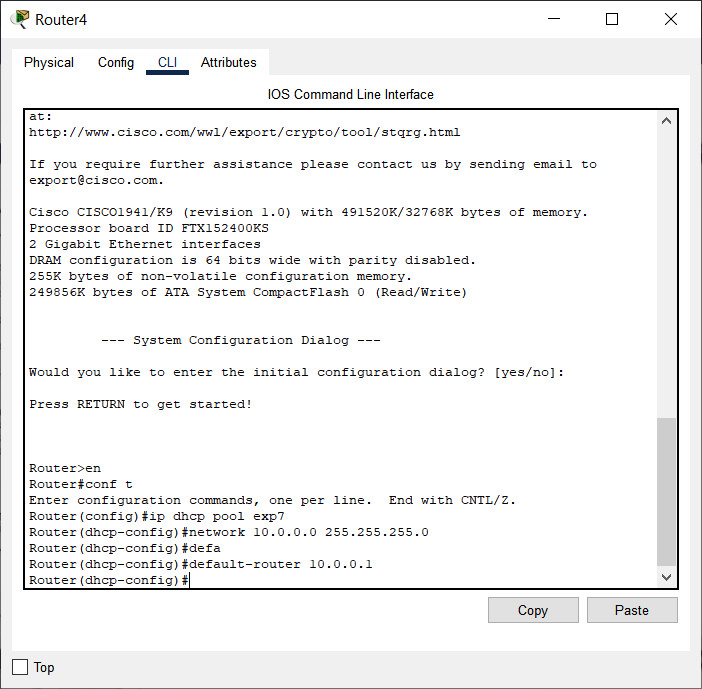
\includegraphics[width=0.5\columnwidth]{figs/s-3-router-server.jpg}
	\caption{دستورات وارد‌شده در روتر سرور}
	\label{fig:s-3-router-server}
\end{figure}

حالا در سمت کلاینت مطابق شکل \ref{fig:s-3-router-client} با اجرای دستور \code{show ip interface brief} می‌بینیم که در ابتدا هیچ ‌آدرسی  برای این روتر وجود ندارد. 
پس با وارد شدن به \lr{interface Gig0/0} و اجرای دستور \code{ip adderess dhcp} آدرس \code{10.0.0.2} به روتر داده می‌شود.
که می‌توان با اجرای دستورات \code{show ip interface brief} و \code{show ip route} هم آن را مشاهده کرد. (شکل \ref{fig:s-3-router-client-brief})

\begin{figure}[h!]
	\centering
	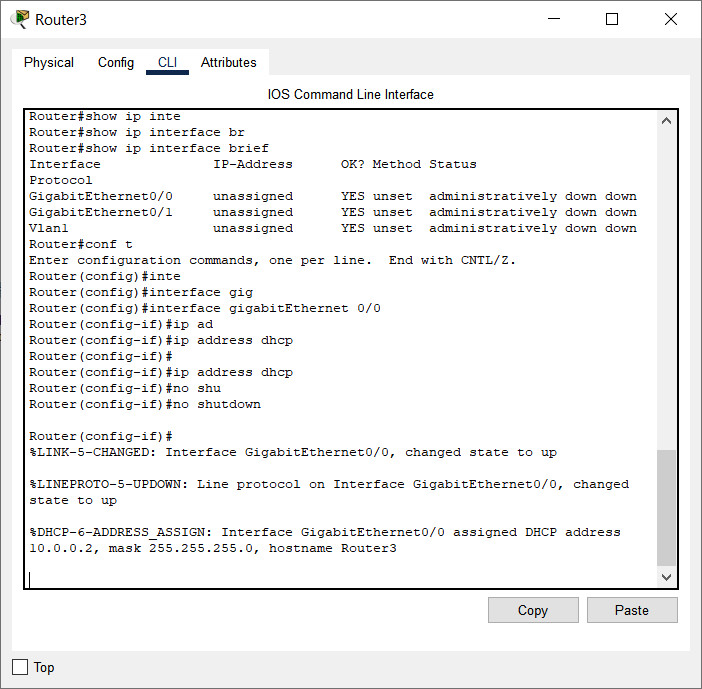
\includegraphics[width=0.5\columnwidth]{figs/s-3-router-client.jpg}
	\caption{دستور تعیین \lr{ip} در کلاینت}
	\label{fig:s-3-router-client}
\end{figure}

\begin{figure}[h!]
	\centering
	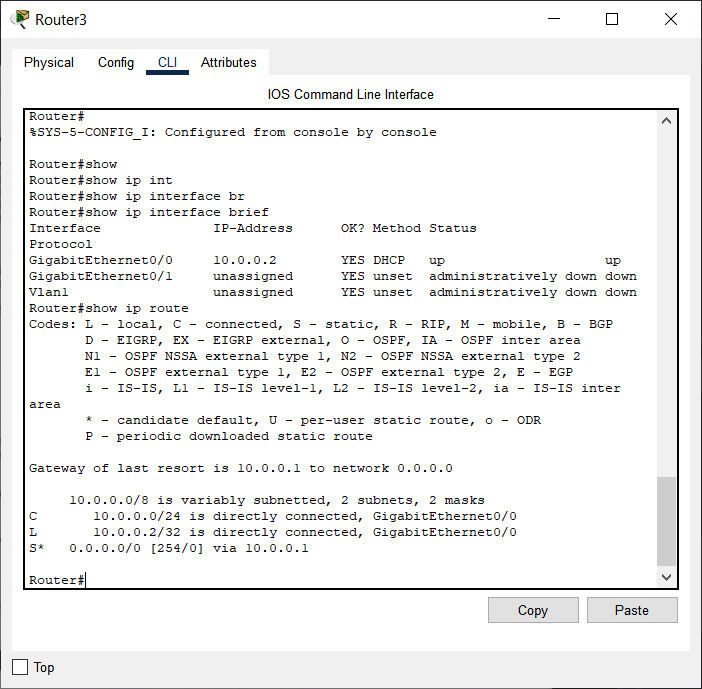
\includegraphics[width=0.5\columnwidth]{figs/s-3-router-client-brief.jpg}
	\caption{مشاهده \lr{ip} داده‌شده توسط \lr{DHCP}}
	\label{fig:s-3-router-client-brief}
\end{figure}



\end{document}
